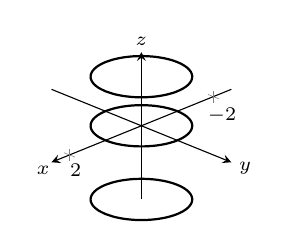
\begin{tikzpicture}[>=stealth]
\begin{axis}%
[width=175pt,tick label style={font=\scriptsize},axis on top,
			axis lines=center,
			view={135}{35},
			name=myplot,
			%xtick={2},
			ytick=\empty,
			ztick=\empty,
			ymin=-2.5,ymax=2.5,
			xmin=-2.5,xmax=2.5,
			zmin=-1.5, zmax=1.5,
			every axis x label/.style={at={(axis cs:\pgfkeysvalueof{/pgfplots/xmax},0,0)},xshift=-3pt,yshift=-3pt},
				xlabel={\scriptsize $x$},
			every axis y label/.style={at={(axis cs:0,\pgfkeysvalueof{/pgfplots/ymax},0)},xshift=5pt,yshift=-2pt},
				ylabel={\scriptsize $y$},
				every axis z label/.style={at={(axis cs:0,0,\pgfkeysvalueof{/pgfplots/zmax})},xshift=0pt,yshift=4pt},
				zlabel={\scriptsize $z$}
			]



%\addplot3[domain=-2:2,,y domain=-2:2,surf,faceted color={\coloronefill},samples=10,colormap={mp2}{\colormapplaneone}] {(x^3-2*x)};

%\addplot3[domain=0:360,,y domain=0:360,surf,faceted color={\coloronefill},samples=30,colormap={mp2}{\colormapplaneone},z buffer=sort] ({cos(x)},{sin(x)*cos(y)},{sin(x)*sin(y)});

%\addplot3[domain=-1.4:1.4,smooth,y domain=-2:2,surf,%fill=white,
colormap={mp2}{\colormapplaneone},faceted color=black!40,samples=10,,z buffer=sort] ({2},{y},{x});

\addplot3[domain=0:360,,thick,smooth,samples y=0,{\colorone},%surf,%fill=white,
samples=30,] ({cos(x)},{sin(x)},{0});

\addplot3[domain=0:360,,thick,smooth,samples y=0,{\colorone},%surf,%fill=white,
samples=30,] ({cos(x)},{sin(x)},{-1.5});

\addplot3[domain=0:360,,thick,smooth,samples y=0,{\colorone},%surf,%fill=white,
samples=30,] ({cos(x)},{sin(x)},{1});

\end{axis}

\end{tikzpicture}











